\documentclass[t, aspectratio=169]{beamer}
\usepackage{amsmath,amsfonts,amsthm,amstext,amssymb, xcolor, tikz, pgf, mathrsfs, polynom, pifont, tabto}

% ----------------------------------------------------------
% Theme Setup

% Use Metropolis Theme
\usetheme[numbering=fraction]{metropolis}
\setbeamertemplate{blocks}[rounded][shadow=false]
\makeatletter
\setlength{\metropolis@titleseparator@linewidth}{1pt}
\makeatother

% Define Colors
\definecolor{chargerblue}{HTML}{002764}
\definecolor{chargerred}{HTML}{e02034}
\definecolor{bggray}{HTML}{d0d3d4}

% Set Colors
\setbeamercolor{title}{fg=chargerblue}
\setbeamercolor{background canvas}{bg=white}
\setbeamercolor{title separator}{fg=chargerred}
\setbeamercolor{structure}{fg=chargerblue}
\setbeamercolor{frametitle}{fg=white, bg=chargerblue}
\setbeamercolor*{normal text}{fg=chargerblue}
\setbeamercolor*{block body}{bg=bggray}
\setbeamercolor*{block title}{bg=chargerblue, fg=white}
% ----------------------------------------------------------

% ----------------------------------------------------------
% Custom Definitions, Commands, Environments, etc.

% Sets of numbers
\def\R{\mathbb{R}} % The reals
\def\N{\mathbb{N}} % The naturals
\def\Z{\mathbb{Z}} % The integers
\def\Q{\mathbb{Q}} % The rationals

% Blank space
\newcommand{\blank}[1]{\underline{\hspace{#1}}} % Blank space

% Change font colors
\newcommand{\cyan}[1]{{\color{cyan}{#1}}} % Changes font to cyan
\newcommand{\red}[1]{{\color{red}{#1}}} % Changes font to red
\newcommand{\magenta}[1]{{\color{magenta}{#1}}} % Changes font to magenta
\newcommand{\orange}[1]{{\color{orange}{#1}}} % Changes font to orange
\newcommand{\yellow}[1]{{\color{yellow}{#1}}} % Changes font to yellow
\newcommand{\violet}[1]{{\color{violet}{#1}}} % Changes font to violet
\newcommand{\green}[1]{{\color{green}{#1}}} % Changes font to green
\newcommand{\blue}[1]{{\color{blue}{#1}}} % Changes font to blue
\newcommand{\white}[1]{{\color{white}{#1}}} % Changes font to white

% Fitted inclusion symbols
\newcommand{\fp}[1]{\left({#1}\right)} % Fitted parentheses around content
\newcommand{\fb}[1]{\left[{#1}\right]} % Fitted brackets
\newcommand{\lhoi}[1]{\left({#1}\right]} % Left half-open interval
\newcommand{\rhoi}[1]{\left[{#1}\right)} % Right half-open interval
\newcommand{\set}[1]{\left\{{#1}\right\}} % Fitted braces (useful for sets)
\newcommand{\av}[1]{\left|{#1}\right|} % Fitted absolute value bars

% Augmented Matrix Environment
\newenvironment{amatrix}[1]{%
	\left[\begin{array}{@{}*{#1}{c}|c@{}}
	}{%
	\end{array}\right]
}

% Miscellaneous
\def\then{\Rightarrow}
\def\to{\rightarrow}
\def\d{^{\circ}}
\newcommand{\?}{\stackrel{?}{=}}
\newcommand{\cmark}{\text{ \ding{51}}}
\newcommand{\xmark}{\text{ \ding{55}}}
\newcommand{\nCr}[2]{\,_{#1}C_{#2}} % nCr
\newcommand{\nPr}[2]{\,_{#1}P_{#2}} % nPr

% Coordinate Plane (Four-Quadrant)
\def\coordplane {
	\begin{tikzpicture}        \draw[step=0.25cm,black,very thin,opacity=0.25] (-2.5cm, -2.5cm) grid (2.5cm, 2.5cm);
		\draw[<->,thick,black] (-2.5cm, 0) -- (2.5cm, 0) node[anchor=north west,pos=0.94,font=\scriptsize]{$x$};
		\draw[<->,thick,black] (0,-2.5cm) -- (0, 2.5cm) node[anchor=south east,font=\scriptsize,pos=0.94]{$y$};
	\end{tikzpicture}
}

% Coordinate Plane (One-Quadrant)
\def\onequad {
	\begin{tikzpicture}
		\draw[step=0.25cm, black, very thin, opacity=0.25] (0,0) grid (7.5cm,5cm);
		\draw[->, thick, black] (0,0) -- (7.5cm, 0) node[anchor=north west,font=\scriptsize,pos=0.94]{$x$};
		\draw[->, black, thick] (0,0) -- (0,5cm) node[anchor=south east,font=\scriptsize,pos=0.94]{$y$};
	\end{tikzpicture}
}
% ----------------------------------------------------------

% ----------------------------------------------------------
% Presentation Information
\title[5-3]{The Binomial Distribution}
\subtitle{Section 5-3}
\author{Jacob Ayers}
\institute{Lesson \#16}
\date{MAT 110}
% ----------------------------------------------------------

\begin{document}
	
	% Slide 1 (Title Slide)
	\begin{frame}
		\titlepage
	\end{frame}
	
	% Slide 2 (Objectives)
	\begin{frame}{Objectives}
		\begin{itemize}
			\item Find probabilities in binomial distributions
			\item Find the mean, variance, and standard deviation of a variable in a binomial distribution
		\end{itemize}
	\end{frame}

	\begin{frame}{Binomial Experiments}
		Many experiments only have two outcomes, or can be reduced to an experiment with two outcomes. \pause
		
		Examples: \begin{itemize}
			\item Tossing a coin (H/T) \pause
			\item Baseball at-bat (get on base or not) \pause
			\item Rolling a die (even or not) \pause
		\end{itemize}
	
		An experiment with two outcomes is called a \textit{binomial experiment}. \pause
		
		Each repetition of the experiment is called a \textit{trial}.
	\end{frame}

	\begin{frame}{Binomial Experiments}
		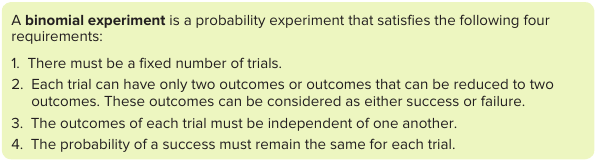
\includegraphics[width=\textwidth]{binom-exp.png} \pause
		
		\textit{Note:} A \textit{success} is not necessarily a positive event!
	\end{frame}

	\begin{frame}{Binomial Experiments}
		Determine whether each experiment is a binomial experiment.
		
		a) Selecting 20 university students and recording their class rank. \\
		b) Selecting 20 students from a university and recording their sex. \\
		c) Drawing five cards from a deck without replacement and recording whether they are red or black. \\
		d) Selecting five students from a large school and asking them if they are on the dean's list. \pause
		
		a) No. There are more than two possible class ranks (Fr., So., Jr., Sr.) \pause \\
		b) Yes. All criteria are met. \pause \\
		c) No. Events aren't independent since cards aren't replaced. \pause \\
		d) Yes. All criteria are met.
	\end{frame}

	\begin{frame}{Binomial Distributions}
		The outcomes of a binomial experiment and the corresponding probabilities of these outcomes is a \textit{binomial distribution}. \pause
		
		Outcomes are usually called successes or failures. \pause
		
		Example: Guessing on a multiple-choice question on a test. \pause
		
		There are two outcomes - right or wrong. \pause
		
		Being right would be considered a success, while being wrong would be considered a failure.
	\end{frame}

	\begin{frame}{Probability and Binomial Distributions}
		To find the probability of exactly $X$ successes in $n$ trials of a binomial experiment, use the formula $$P(X) = \nCr{n}{X}  \cdot p^X \cdot q^{n-x}$$ where
		
		$p$ is the probability of success \\
		$q$ is the probability of failure \pause (note: $q = 1 - p$) \pause
		
		A graphing calculator can also find these probabilities.
	\end{frame}

	\begin{frame}{Probability and Binomial Distributions}
		A survey found that one out of five Americans says he or she has visited a doctor in any given month. If 10 people are selected at random, find the probability that half of them have visited a doctor last month.
		
		\onslide<2->{This is a binomial distribution, with the following parameters:} \\
		\onslide<3->{$n = 10$} \\
		\onslide<4->{$X = 5$ (half of 10)} \\
		\onslide<5->{$p = 0.20$ ($1 \div 5$)} \\
		\onslide<6->{$q = 1 - 0.20 = 0.80$} \begin{flalign*}
			\onslide<7->{P(X) &= \nCr{n}{X} \cdot p^X \cdot q^{n-X} & \\}
			\onslide<8->{P(5) &= \nCr{10}{5} \cdot (0.20)^5 \cdot (0.80)^{10 - 5} & \\}
			\onslide<9->{&\approx 0.026}
		\end{flalign*}	
	\end{frame}

	\begin{frame}{Probability and Binomial Distributions}
		Twenty-six percent of couples who plan to marry this year are planning destination weddings. In a random sample of 12 couples who plan to marry, find the probability that \begin{enumerate}[a)]
			\item Exactly 4 of them are planning destination weddings.
			\item No more than 3 of them are planning destination weddings.
			\item At least 8 of them are planning destination weddings.
		\end{enumerate} \pause
	
		In each situation, we have that $n = 12$, $p = 0.26$, and $q = 1 - 0.26 = 0.74$. \pause
		
		a) $P(4) = \nCr{12}{4} \cdot (0.26)^4 \cdot (0.74)^8 \approx 0.203$
	\end{frame}

	\begin{frame}{Probability and Binomial Distributions}
		b) We have a couple ways of finding $P(\text{no more than 3})$: \pause
		
		$P(0) + P(1) + P(2) + P(3)$ \pause OR $1 - (P(4) + P(5) + \cdots + P(12))$ \pause
		
		The first option will be faster so I'll do it that way.
		
		$P(0) = \nCr{12}{0} \cdot 0.26^0 \cdot 0.74^{12} \approx 0.02696$ \\ \pause
		$P(1) = \nCr{12}{1} \cdot 0.26^1 \cdot 0.74^{11} \approx 0.11369$ \\ \pause
		$P(2) = \nCr{12}{2} \cdot 0.26^1 \cdot 0.74^{10} \approx 0.21969$ \\ \pause
		$P(3) = \nCr{12}{3} \cdot 0.26^3 \cdot 0.74^{9} \approx 0.25729$ \\ \pause
		
		Adding these values: $P(\text{no more than 3}) = 0.02696 + 0.11369 + 0.21969 + 0.25729 \approx 0.618$ \pause
		
		Calculator Shortcut: Use $binomcdf(12,.26,3)$. \pause
		\textit{CDF} is short for \textit{cumulative density function}. It finds the probability that the number of successes will be less than or equal to a given number.
	\end{frame}

	\begin{frame}{Probability and Binomial Distributions}
		Fifty-three percent of all persons in the US population have at least some college education. Choose 10 persons at random. Find the probability that at least 7 of them have at least some college education.
		
		Once again, we have options:
		
		$P(\text{at least 7}) = P(7) + P(8) + P(9) + P(10)$ \pause OR \\
		$P(\text{at least 7}) = 1 - \fp{P(0) + P(1) + \cdots + P(6)}$ \pause
		
		$P(7) + P(8) + P(9) + P(10) \approx 0.14635 + 0.06189 + 0.01551 + 0.00017 \approx 0.226$ \pause
		
		If we use the binomial cdf shortcut, the second method is actually faster. \pause
		
		$P(\text{at least 7}) = 1 - binomcdf(10, 0.53, 6) \approx 0.226$	
	\end{frame}

	\begin{frame}{Mean, Variance, and Standard Deviation of Binomial Distributions}
		We could find the mean, variance and standard deviation the way we learned in the last lesson, but that would require us to make the entire probability distribution. \pause
		
		Fortunately, there are simple shortcut formulas we can use instead. \pause
		
		Mean: $\mu = np$ \\
		Variance: $\sigma^2 = npq$ \\
		Standard Deviation: $\sigma = \sqrt{npq}$
	\end{frame}

	\begin{frame}{Mean, Variance, and Standard Deviation of Binomial Distributions}
		The \textit{Sourcebook of Criminal Justice Statistics} states that 65\% of Americans favor sentencing drunk drivers to jail even if they have not caused an accident. If 1000 individuals are selected at random, find the mean, variance, and standard deviation of the people who feel this way. \pause
		
		$\mu = 1000 \cdot 0.65 = 650$ \\ \pause
		$\sigma^2 = 1000 \cdot 0.65 \cdot 0.35 = 227.5$ \\ \pause
		$\sigma = \sqrt{227.5} \approx 15.1$
	\end{frame}

	\begin{frame}{Mean, Variance, and Standard Deviation of Binomial Distributions}
		Thirty-two percent of adult Internet users have purchased products or services online. For a random sample of 200 adult Internet users, find the mean, variance and standard deviation for the number who have purchased goods or services online.
		
		$\mu = 200 \cdot 0.32 = 64$ \\ \pause
		$\sigma^2 = 200 \cdot 0.32 \cdot 0.68 = 43.52 \approx 43.5$ \\ \pause
		$\sigma = \sqrt{43.52} \approx 6.6$
	\end{frame}

	\begin{frame}{Next Steps}
		\begin{itemize}
			\item Read 6-1
			\item Watch Video Lesson \#17
			\item Complete Assignment 8
		\end{itemize}
	
		\vfill
		
		Thanks for watching!
	\end{frame}
	
\end{document}